\subsection{Pipeline: Proposed Model (Detailed View)}
Our proposal of combined workflows suggests an amalgamation of tasks condensed into three major steps: (1) MRI data preparation, (2) colour mapping, and (3) hologram encoding.  The MRI data preparation involved the extraction of a MRI DICOM or NIFTI medical file of 181 slices for our brain, after which we applied segmentation to isolate the tumour in the image data in traditional DICOM GSDF grayscale.  The colour mapping process was applied to the volume data, and tests show that a divergent and/or structured colormap yield preferred results of highlighting image detail.

\begin{figure}[t]
 \centering % avoid the use of \begin{center}...\end{center} and use \centering instead (more compact)
 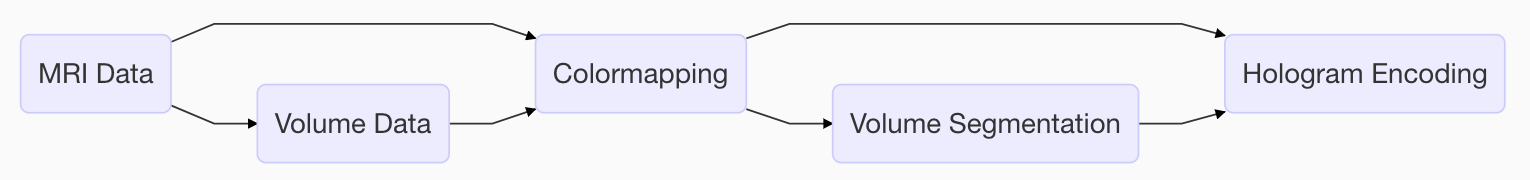
\includegraphics[width=\columnwidth]{pictures/proposed-model.png}
 \caption{Proposed pipeline model}
 \label{fig:proposed-model}
\end{figure}